\section{Introduction}
\vspace{-3mm}
Big data technologies have affected every corner of human life and society. These technologies have made our lives unimaginably more shared,  connected,  convenient,  and cost-effective. Using data-driven technologies gives us the ability to make wiser decisions, and can help make society safer, more equitable and just, and more prosperous.
However, while having an enormous potential to help solve societal issues, 
{\em irresponsible} implementation of these technologies  can not only fail to help, but may even make matters worse.  
%The reason that data ethics has caught a lot of recent attention is that big data technologies constantly fail to fulfill their promise of solving our societal issues. 
Racial bias in predictive policing and data-driven judgeship, harming marginalized people and poor communities, and sexism in job recommendation systems are a few examples of such failures. In order to minimize societal harms of data-driven technologies, and to ensure that objectives such as fairness, equity, diversity, robustness, accountability, and transparency are satisfied, it is necessary to
develop proper {\em tools, strategies, and metrics}. 
% This is our ultimate objective. To this end, we propose Mithra, an assistive toolbox that help data scientists conduct data-driven tasks, responsibly. 
% That is, to assure data ethics norms are satisfied, while making data-driven decisions.

Human decision makers often receive assistance from data-driven algorithmic systems that {\em provide a score for evaluating objects, including individuals}.
The scores can be computed by combining different attributes either through a process learned by ML models (using some training data),  or using a weight vector assigned by human experts.  For example, a support vector machine learns the parameter values that define a linear separator in some regularized multi-dimensional feature space.  Learning methods require that there be labeled data, and assume that there is some known ground truth. 
% In practice, we may not really know.  For example, any quantitative performance metric is only an approximate reflection of the value of an employee hired or a student admitted.  Maximizing this metric doesn't necessarily maximize what we really care about.


\begin{wrapfigure}{r}{0.4\textwidth}
%\vspace{-9mm}
    \begin{center}
    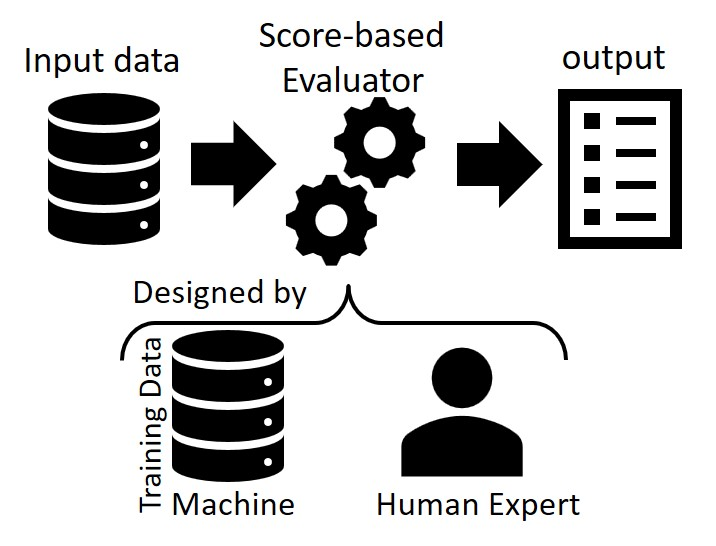
\includegraphics[width=\linewidth]{figs/ScoringArch.jpg}
    \end{center}
%    \vspace{-10mm}
    \caption{General architecture of score-based systems}
    \label{fig:DSSArch}
    %\vspace{-3mm}
\end{wrapfigure}

\noindent In contrast, an expert-specified method does not require any labeled data, but may be ad-hoc.
The scores are used either to evaluate an object independently (by only looking at its score) or in comparison with others. 

Two major categories of methods that use scores to supporting decisions are (i) {\em Classification} and (ii) {\em Ranking}\footnote{Note that in some contexts ranking or classification is done without scoring. For instance,
rank aggregation from partial ranked lists~\cite{marcus2011human} or pairwise comparisons~\cite{asudeh2015pareto} is popular for group opinion collection.  Our focus in this paper are evaluations (including ranking and classification) based on scores.
}.
%Figure~\ref{fig:rankingvsclassification} show a comparison between these two. 
Classification is often used for predicting future outcomes based on historical data.
Predicting recidivism and classifying individuals based on how likely they will commit a crime in the future is a societally important example of this kind.
Ranking, on the other hand, is used for assignment by comparison on the existing data.
For example, a company may rank its employees, and then reward high-ranked employees (with a raise or promotion) and fire low-ranked employees. College admissions is another example where the top-$k$ applicants may be admitted by a college.
Similarly, the international football association FIFA considers its rankings as ``a reliable measure'' for seeding the international tournaments such as the World Cup~\cite{fifa}.

Rankings are relative while labels in classification are absolute. That is, the rank of an individual depends on the others in the dataset, while class labels are assigned solely based on the score of an individual.
The scoring mechanism for classification is usually learned by ML models. It can be a linear model such as regression and SVM, or a complex deep learning model.  On the other hand, %since ranks of items are relative,  (hence it is not possible to have labeled data)
scoring mechanism for ranking is usually designed by human experts. US News university rankings, FIFA rankings, and CSRankings\footnote{\small csrankings.org} are some of these examples.

Of course, the dichotomy above is not as clean as the preceding paragraph may suggest. Not all classification scoring is machine-learned. For example PSA (Public Safety Assessment) scores\footnote{\small www.psapretrial.org/about/factors}, used in data-driven judgeship, are human-designed.  Similarly, ranking can be the basis for classification through the introduction of a cut-off rank, as in the case of college admissions.

% \begin{figure*}[!tb]
% %\begin{minipage}[t]{0.6\textwidth}
% %\centering
% %\vspace{-39mm}
% %    \begin{tabular}{|@{}l@{}||@{}c@{}|@{}c@{}|}
% %    \hline
% %        &{\bf Ranking} & {\bf Classification} \\ \hline\hline
% %        \textit{Objective} &  Assignment & Predicting\\ 
%  %       & by comparison$~$ & future outcomes\\ \hline
% %        \textit{Scoring Model } & Usually linear & Linear or complex\\ \hline
%  %       \textit{Designed by} & Human Experts & Usually Machine learning\\ \hline
%  %       \textit{Relativity}&Ranks are & Class labels\\
% %        &relative & $~$are absolute\\ \hline
% %   \end{tabular}
% %   \caption{Ranking vs. Classification}
% %   \label{fig:rankingvsclassification}
% %\end{minipage}
% %\hfill
% \begin{minipage}[t]{0.39\textwidth}
% \centering
%     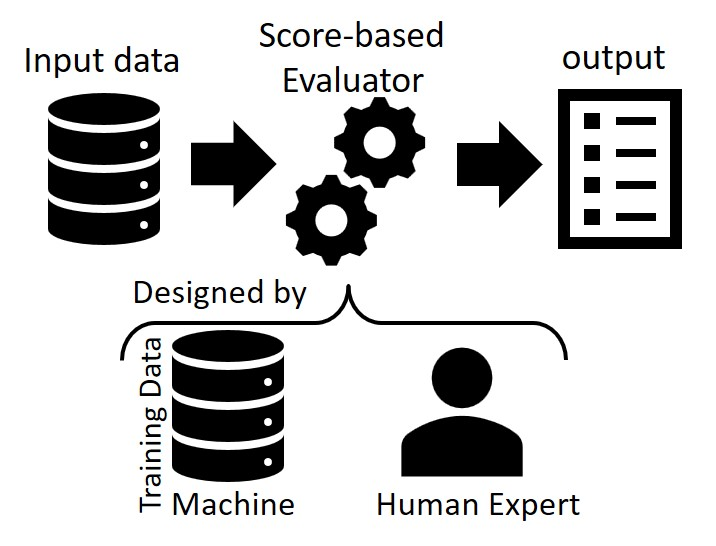
\includegraphics[width=0.9\textwidth]{figs/ScoringArch.jpg}
%     \vspace{-6mm}\caption{General architecture of score-based systems}
%     \label{fig:DSSArch}
% \end{minipage}
% \vspace{-6mm}
% \end{figure*}

Figure~\ref{fig:DSSArch} shows the general architecture of score-based systems for data-driven decision making.
The central component in these systems are the score-based evaluators that assign a score to each individual in the input data and generate the output by, for example, ranking or classifying the input. The output provides the evaluation of individuals that is used for decision making. %Also, as mentioned previously, 
Note that 
the scoring module can be designed by experts, or be learned by a machine, using some training data.

% Mithra is our project for responsible data-driven decision making.
We, in our project Mithra, view \textit{human experts} (for human-designed evaluators) and \textit{training data} (for machine learned evaluators) as the keys to achieving responsibility in score-based systems.
That is, for human-designed tasks such as ranking, we advocate designing assistive tools that help experts make sure their evaluators meet the objectives of fairness and stability. On the other hand, for machine learning tasks such as classification, we advocate assessing and repairing training data to make sure that, for example,  the data is representative of minority groups~\cite{asudeh2019designing}, and models trained on that data do not reflect results of historical discrimination~\cite{salimi2019capuchin2}.
In the following, first in \S~\ref{sec:ranking}, we explain our research for score-based ranking. Then in \S~\ref{sec:coverage}, we provide our results for machine learning tasks such as classification by assessing and enhancing coverage for a (given) training dataset.



% We view human experts, the central component the design of 

% In general the approaches to make data-driven decision making ethical target 
% (i) assessing and repairing the training data~\cite{asudeh2019assessing,salimi2019capuchin,}, (ii) the design of evaluators~\cite{asudeh2019designing,asudeh2018obtaining,}, and (iii) the output of evaluators~\cite{yang2018nutritional}.
% We focus on responsible design of evaluators and advocate data assessment and repair.
% We, however, do not consider direct manipulation of output data and disparate treatment.
% The main concentration of Mithra has been on score-based evaluator, especially ranking. 

